\documentclass[12pt, aspectratio=169]{beamer}

\usepackage{color}
\usepackage[utf8]{inputenc}
\usepackage{graphicx}
\usepackage{tikz}
\usepackage[T1]{fontenc}
\usepackage{caption}
\usepackage{wrapfig}
\usepackage{xurl}

\captionsetup[figure]{labelformat=empty}
\setbeamertemplate{section in toc}[square]
\usefonttheme[onlymath]{serif}

\usetheme{Singapore}
\usecolortheme{default}
\usefonttheme{structurebold}
\setbeamerfont{text}{size=\large}
\setbeamertemplate{bibliography item}{\insertbiblabel}

\definecolor{ao}{rgb}{0.0, 0.0, 0.7}


\setbeamercolor{block body alerted}{bg=alerted text.fg!10}
\setbeamercolor{block title alerted}{bg=alerted text.fg!20}
\setbeamercolor{block body}{bg=structure!10}
\setbeamercolor{block title}{bg=structure!20}
\setbeamercolor{block body example}{bg=green!10}
\setbeamercolor{block title example}{bg=green!20}

\newcommand{\nimadd}{\overset{*}{+}}

%\setbeamertemplate{footline}[frame number]
\setbeamertemplate{footline}[text line]{%
  \parbox{\linewidth}{\vspace*{-8pt}\color{ao}\insertshorttitle\hspace{10px}\insertshortauthor\hfill\insertpagenumber}}

\title{Kombinatorische Spieltheorie}
\author[Y. Höll]{Yannik Höll}
\date{3. März, 2023}
% \logo{
\includegraphics[keepaspectratio=True, width=30px]{./image/logo.png}}

\beamertemplatenavigationsymbolsempty 

\begin{document}
\begin{frame}[noframenumbering, plain]
	\titlepage
\end{frame}

\begin{frame}
	\frametitle{Einteilung}
	\tableofcontents
\end{frame}

\section{Einleitung}
\begin{frame}
    \frametitle{Kombinatorische Spiele}
    Kombinatorische Spieltheorie beschäftigt sich mit Spielen die:

\begin{itemize}
    \item 2 Spieler (Links, Rechts)
    \item endliche/abzählbare Positionen
    \item Spieler ziehen abwechselnd
    \item jeder Spieler hat vollständige Information
    \item kein Zufall
    \item Konvention: Keine Züge mehr $\Rightarrow$ Verlierer (kein Unentschieden)
\end{itemize}

\onslide<2-> {
Kombinatorische Spieltheorie ist:
\begin{itemize}
    \item nicht wie gewöhnliche Spieltheorie
    \item eher mathematische Rätsel, Denkaufgaben
\end{itemize}
}
\end{frame}

\begin{frame}
\frametitle{Kombinatorische Spiele}

Nicht untersucht werden können Spiele wie:
\begin{itemize}
    \item<2-> Schach (Unentschieden)
    \item<3-> Backgammon (Zufall)
    \item<4-> Tennis, oder andere Sportarten (keine diskreten Zustände)
    \item<5-> Schere-Stein-Papier (keine vollständige Information, nicht abwechselnd)
\end{itemize}

\onslide<6-> {
    $\Rightarrow$ viele untersuchte Spiele eher unbekannt \\
    $\Rightarrow$ Die meisten Spiele wurden wegen Theorie "erfunden"
}
\end{frame}

\begin{frame}
    \frametitle{Kombinatorische Spieltheorie}
    \centering
    \huge{\textbf{Zentrale Frage:} Gibt es eine Strategie, durch die einer der beiden Spieler sicher gewinnt?}
\end{frame}

\section{Nim}

\begin{frame}
    \frametitle{Nim}
    \textbf{Regeln}:
    \begin{itemize}
        \item<1-> Stapel mit Münzen
        \item<1-> Spieler entfernen beliebig viele Münzen von beliebigem Stapel
        \item<1-> Keine Unterscheidung der Spieler
        \item<2-> Spiel heißt "Impartial" 
    \end{itemize}
    \begin{figure}
        \centering
        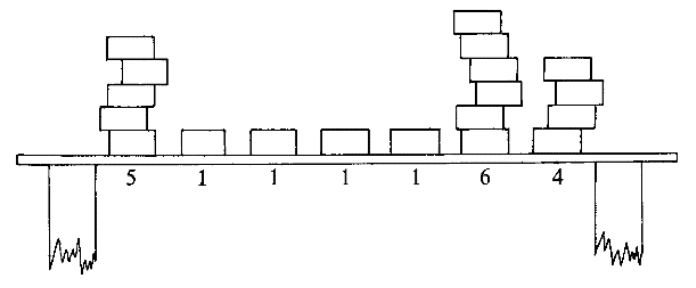
\includegraphics[width=0.6\textwidth]{pic/nim-pos.png}
        \caption{Eine Nim-Position \tiny{\cite{ww}}}
    \end{figure}
\end{frame}

\begin{frame}
    \frametitle{Nim}
    $n,k \in \mathbb{N}$:
    \begin{itemize}
        \item<1-> Position ohne Münze ($N_{0}$): Zweiter Spieler gewinnt
        \item<2-> Position mit einem Turm($N_{k}$): Erster Spieler gewinnt
        \only<2-2>{\item Position mit mit 2 Türmen mit gleicher Anzahl an Münzen($N_{k,k}$): \\ \textbf{Hypothese:} 2. Spieler gewinnt immer, indem er den Gegner nachahmt }
        \item<3-> Position mit mit 2 Türmen mit gleicher Anzahl an Münzen: \\ 2. Spieler gewinnt immer, indem er den Gegner nachahmt
        \item<4-> Position mit mit 2 Türmen mit unterschiedlicher Anzahl an Münzen ($N_{n,k}, n > k$): \\ 1. Spieler gewinnt immer, indem er $N_{n,k}$ nach $N_{k,k}$ überführt
    \end{itemize}
\end{frame}

\begin{frame}
    \frametitle{Nimbers}
    \begin{itemize}
        \item<1-> \textbf{Def:} $0$ = Spiel, bei dem der 2. Spieler gewinnt
        \item<2-> $*k$ = Nim-Turm mit $k \in \mathbb{N}$ Münzen 
        \item<3-> $*k + *k = 0 \Rightarrow *k = - (*k)$
        \item<4-> $* + (*2) + (*3) = 0 \Rightarrow * + (*2) = *3$
        \item<4-> \textbf{Aber}: $* + (*3) = (*2)$, $(2*) + (*3) = *$
        \item<4-> Nim-Addition verhält sich nicht wie Addition in $\mathbb{N}$
        \item<5-> Allgemeine Nim-Addition entspricht der vollständigen Nim-Theorie
    \end{itemize}
    
\end{frame}

\begin{frame}
    \frametitle{Nim-Addition}
    \begin{block}{Allgemeine Nim-Addition}
        \centering
        $*m + *n = *k$: $*k \neq *m' + *n$ und $*k \neq *m + *n'$ \\ mit $n' < n$ und $m' < m$
    \end{block}
    \onslide<2-> {
    $\Rightarrow \forall k \in \mathbb{N}: n < 2^k \Rightarrow *2^k + *n = *(2^k + n)$ \\
    }
    \onslide<3-> {
    $\Rightarrow \forall k,n \in \mathbb{N}: k \neq n: *2^k + *2^n = *(2^k + 2^n)$ \\
    $\Rightarrow \forall k \in \mathbb{N}: *2^k + *2^k = 0$ \\
    }
    \onslide<4-> {
        \vspace*{20px}
        \alert{Die allgemeine Nim-Addition verhält sich wie eine bitweise XOR-Operation.}
    }
\end{frame}

\begin{frame}
    \frametitle{Nim-Addition - Beispiel}
    \begin{align*}
        5 \nimadd 3 &= (4 + 1) \nimadd (2 + 1) = 4 \nimadd 2 = 4 + 2 = 6 \\
        \onslide<2->{11 \nimadd 22 \nimadd 33 &= (8 + 2 + 1) \nimadd (16 + 4 + 2) \nimadd (32 + 1) = 8 + 16 + 4 + 32 = 60}
    \end{align*}
\end{frame}

\begin{frame}
    \frametitle{Spiel - Abstrakte Definition}

    \begin{block}{Kombinatorisches Spiel}
        \begin{center}
            $G = \{ a,b,c,\cdots | \: d,e,f,\cdots\}$
        \end{center}
        wobei $a,b,c,d,e,f$ Kombinatorische Spiele sind. $a,b,c$ sind die Optionen des ersten Spielers (Links);
        $d,e,f$, die des 2. Spielers (Rechts). 
    \end{block}
    $G = \{G^L | \: G^R\}$, falls es eine beste Optionen $G^L$ für Links und $G^R$ für rechts gibt. \\
    $G^L$ ist beste Option $\iff \forall G^L_i \neq G^L: G^L > G^L_i$
\end{frame}

\begin{frame}
    \frametitle{Spiel - Abstrakte Definition}

    \begin{block}{Addition von Kombinatorischen Spielen}
        $G = \{G^L| \: G^R\}, H = \{H^L | \: H^R\}$ Kombinatorische Spiele$: $
        \[ G+H = \{G^L + H, G + H^L | \: G^R + H, G + H^R\} \]
    \end{block}

    \begin{block}{Inverse von Kombinatorischen Spielen}
        $G = \{G^L| \: G^R\}$ Kombinatorische Spiele:
        \[ -G = \{-G^R |\: -G^L \}\]

    \end{block}

\end{frame}

\begin{frame}
    \frametitle{Spiel - Abstrakte Definition}

    \begin{align*}
        -G &= \{-G^R |\: -G^L \} \\
        \vspace*{100px}\\
        G + (-G) &= \{G^L| \: G^R\} + \{-G^R |\: -G^L \} \\
        &= \{G^L + -G, G + (-G)^L |\: G^R + -G, G + (-G)^R \} \\
        &= \{G^L + (-G), G + (-G^R) |\: G^R + (-G), G + (-G^L) \} \\
        &\Rightarrow G^L + (-G); \:\: G + (-G^R) \:\:\:\:\: G^R + (-G); \:\: G + (-G^L)
    \end{align*}
\end{frame}


\begin{frame}
    \frametitle{Spiel - Abstrakte Definition}
    \begin{block}{Vergleich von Spielen}
    $G, H$ Kombinatorische Spiele:
    
    \begin{align*}
        G > H \iff G + (-H) > 0 \\
        G \geq H \iff G + (-H) \geq 0 \\
        G < H \iff G + (-H) > 0 \\
        G \leq H \iff G + (-H) \leq 0
    \end{align*}
    
    \end{block}
\end{frame}

\begin{frame}
    \frametitle{Spiel - Abstrakte Definition}
    \begin{block}{Umkehrbare Züge}
    $G = \{A,B,C,\cdots | \: D,E,F,\cdots\}, D^L = \{U,V,W\cdots | \: X,Y,Z,\cdots\}$ Kombinatorische Spiele: \\
    \begin{center}
        $\exists D^L \geq G \iff$ D ist umkehrbarer Zug
    \end{center}
    $\Rightarrow G = \{A,B,C,\cdots | D,E,F,\cdots\} = \{A,B,C,\cdots | \: \alert{X,Y,Z,\cdots},E,F\cdots\} = H$
    \end{block}
\end{frame}

\begin{frame}
    \frametitle{Spiel - Abstrakte Definition}
    \begin{figure}
        \centering
        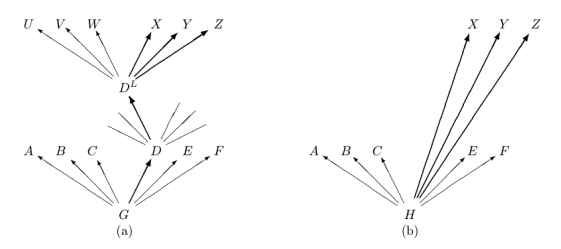
\includegraphics[width=0.8\textwidth]{pic/reversible.png}
        \caption{Schematische Darstellung - Umkehrbarer Zug \tiny{\cite{ww}}}
    \end{figure}
\end{frame}

\begin{frame}
    \frametitle{Beispiel Nim}
    \begin{itemize}
        \item $0 = \{|\}$
        \item $* = \{0|0\}$
        \item $*2 = \{0,*|0,*\}$
        \item $*k = \{0,*,*2,\cdots,*(k-1)|0,*,*2,\cdots,*(k-1)\}$
    \end{itemize}
\end{frame}

\section{Poker-Nim}
\begin{frame}
    \frametitle{Poker-Nim}
    \textbf{Regeln}:
    \begin{itemize}
        \item Alles wie bei Nim
        \item Münzen, die ein Spieler von Stapel wegnimmt, behält der Spieler
        \item statt eine/mehrere Münzen von Stapel zu nehmen, kann Spieler auch Münzen aus seinem "Lager" hinzufügen 
    \end{itemize}
    \begin{center}
        \onslide<2->{\large{Was ist hier eine Gewinnstrategie?}}\\
        \onslide<3->{Bei perfektem Spiel ist Poker-Nim äquivalent zu Nim, da alle nicht-nim Züge umkehrbar sind.}
    \end{center}
\end{frame}

\section{Hackenbush}
\section{Hackenbush-Hotchpotch}

\section{Quellen}
\begin{frame}[allowframebreaks, noframenumbering]
    \nocite{*}
	\hfill
    \bibliographystyle{unsrt}
    \bibliography{references}
\end{frame}


\end{document}